\chapter{Exponential Distribution ($X \sim \exp(\lambda)$) \cite{ism-1,wiki/Exponential_distribution}} \label{Exponential Distribution}

\begin{table}[H]
    \begin{minipage}{0.49\linewidth}
        \begin{figure}[H]
            \centering
            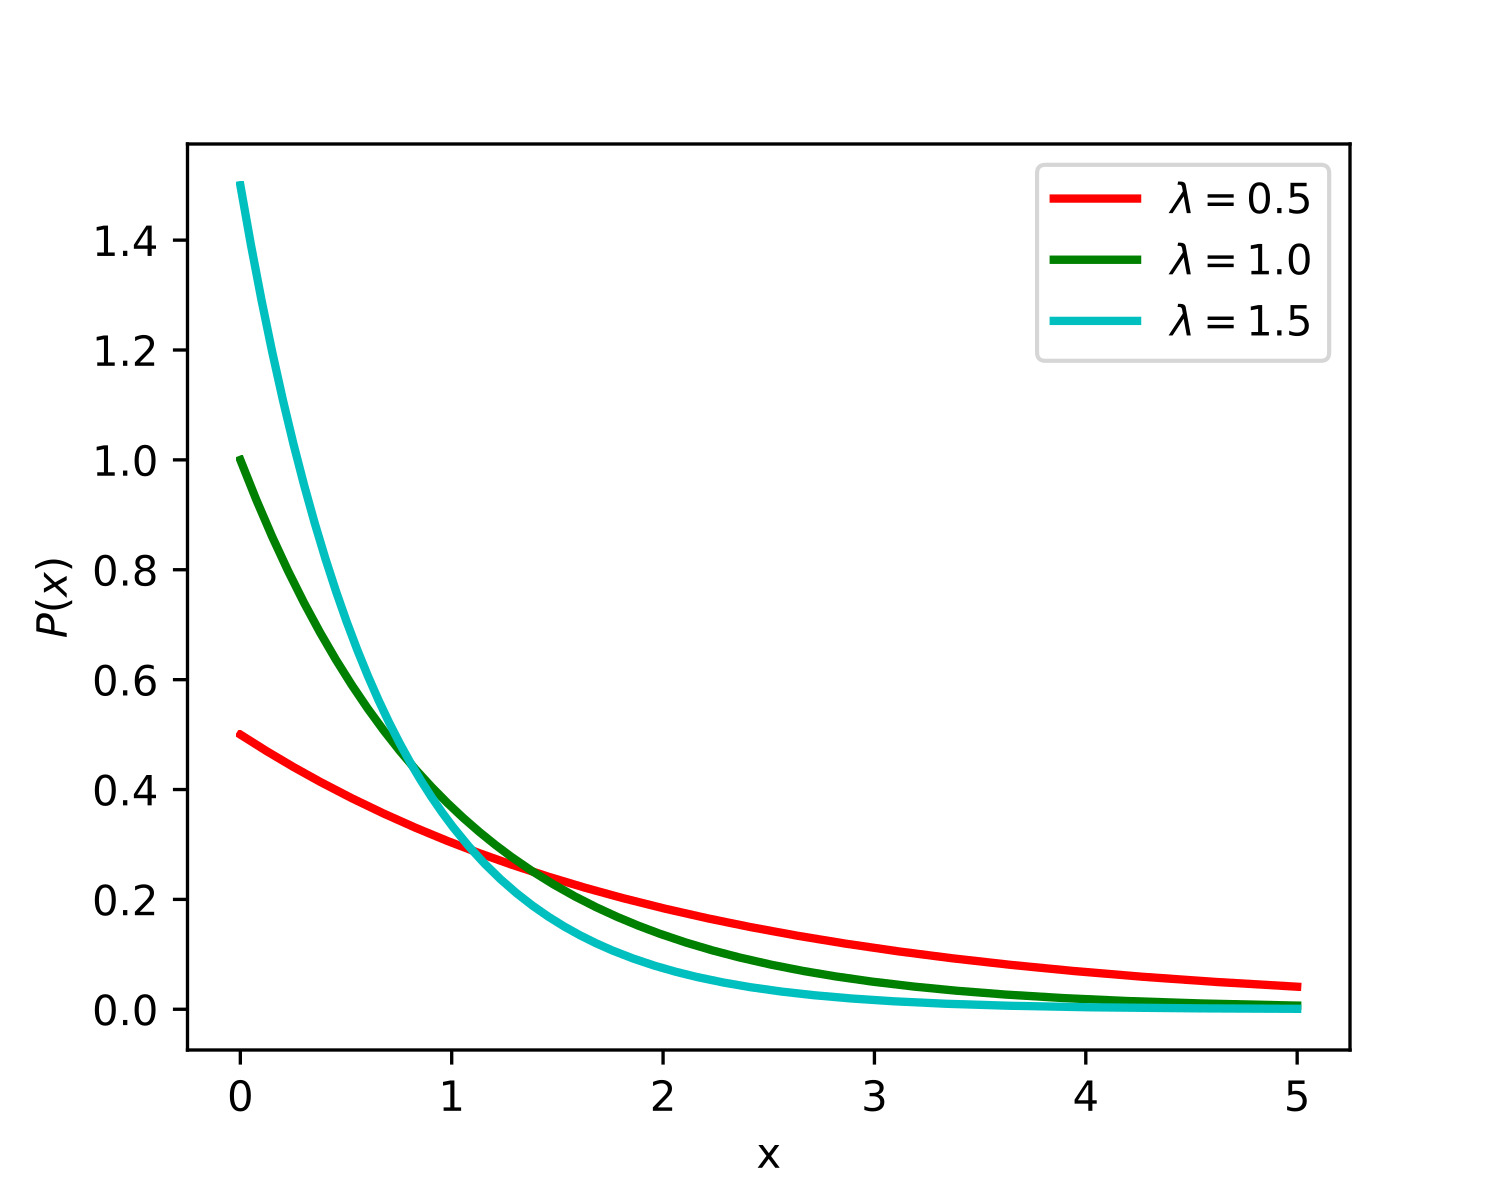
\includegraphics[width=\linewidth, height=4cm, keepaspectratio]{Pictures/distributions/Exponential_distribution_pdf.jpg}
            \caption{Exponential Distribution: PDF}
        \end{figure}
    \end{minipage}
    \hfill
    \begin{minipage}{0.49\linewidth}
        \begin{figure}[H]
            \centering
            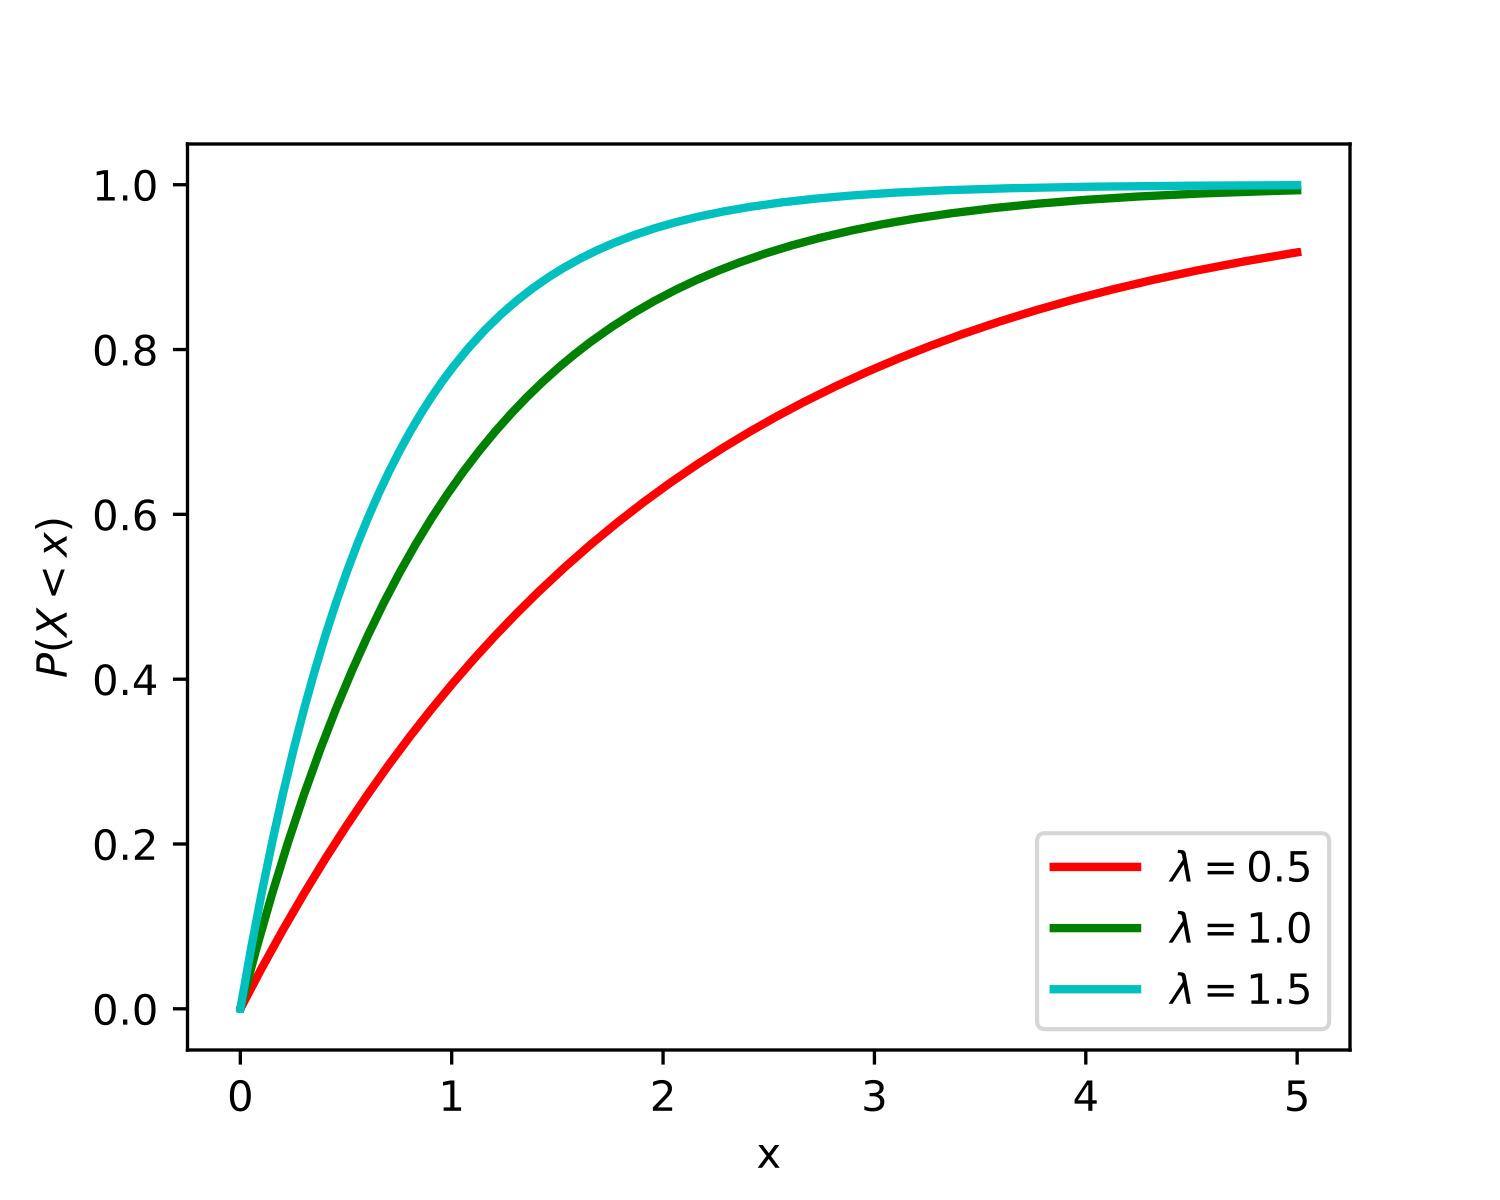
\includegraphics[width=\linewidth, height=4cm, keepaspectratio]{Pictures/distributions/Exponential_distribution_cdf.jpg}
            \caption{Exponential Distribution: CDF}
        \end{figure}
    \end{minipage}
\end{table}

\renewcommand{\arraystretch}{2}
\begin{longtable}{|m{6cm}|p{9cm}|}
    \hline
    \multicolumn{2}{|c|}{\textbf{Exponential Distribution - Info} \cite{wiki/Exponential_distribution}} \\
    \hline\endfirsthead

    \hline
    \multicolumn{2}{|c|}{\textbf{Exponential Distribution - Info - contd.} \cite{wiki/Exponential_distribution}} \\
    \hline\endhead
    
    \hline\endfoot
    \hline\endlastfoot

    \textbf{Statistical parameters} & 
    ${\displaystyle \lambda >0}$ rate, or inverse scale
    \\ \hline
    
    \textbf{Support} &
    ${\displaystyle x\in [0,\infty )}$
    \\ \hline

    \textbf{Probability Density Function (PDF)} & 
    ${\displaystyle \lambda e^{-\lambda x}}$
    \\[1ex] \hline
    
    \textbf{Cumulative distribution function (CDF)} & 
    ${\displaystyle 1-e^{-\lambda x}}$
    \\ \hline

    \textbf{Quantile} &
    ${\displaystyle -{\dfrac {\ln(1-p)}{\lambda }}}$
    \\ \hline

    \textbf{Mean} & 
    ${\displaystyle {\dfrac {1}{\lambda }}}$
    \\[1ex] \hline

    \textbf{Median} & 
    ${\displaystyle {\dfrac {\ln (2)}{\lambda }}}$
    \\[1ex] \hline

    \textbf{Mode} & 
    $0$
    \\ \hline

    \textbf{Variance} &
    ${\displaystyle {\dfrac {1}{\lambda ^{2}}}}$
    \\[1ex] \hline

    \textbf{Skewness} &
    $2$
    \\ \hline

    \textbf{Excess kurtosis} &
    $6$
    \\ \hline

    \textbf{Entropy} &
    ${\displaystyle 1-\ln (\lambda) }$
    \\[1ex] \hline

    \textbf{Moment-generating function (MGF)} &
    ${\displaystyle {\dfrac {\lambda }{\lambda -t}},{\text{ for }}t<\lambda }$
    \\[1ex] \hline

    \textbf{Characteristic function (CF)} &
    ${\displaystyle {\dfrac {\lambda }{\lambda -it}}}$
    \\[1ex] \hline

    \textbf{Fisher information} &
    ${\displaystyle {\frac {1}{\lambda ^{2}}}}$
    \\[1ex] \hline

    \textbf{Kullback–Leibler divergence} &
    ${\displaystyle \ln {\dfrac {\lambda _{0}}{\lambda }}+{\dfrac {\lambda }{\lambda _{0}}}-1}$
    \\[1ex] \hline

    \textbf{Expected shortfall} &
    ${\displaystyle {\dfrac {-\ln(1-p)+1}{\lambda }}}$
    \\[1ex] \hline

    \textbf{Inverse of CDF \cite{ism-1}} &
    $F_\lambda^{-1}(u) = -\dfrac{\log(1-u)}{\lambda}$ $u \in (0,1)$
    \\[1ex] \hline

    \textbf{Relative Standard Deviation} &
    $1$
    \\[1ex] \hline

\end{longtable}
\renewcommand{\arraystretch}{1}


\section{Sample Statistic Minimum ($X_{(1)}$) \cite{ism-1}} \label{Exponential Distribution: Sample Statistic Minimum}

\begin{enumerate}
    \item $F_{X_{(1)}}(x) = 1 - \exp(-n\lambda x)$

    \item The sample distribution of the minimum X(1) is exponentially distributed, 
    \[
        X_{(1)} \sim \exp(n\lambda)
    \]
    but now with parameter $n\lambda$, when $X_1,X_2,\cdots, X_n$ are i.i.d. $exp(\lambda)$ distributed.
    
\end{enumerate}


\section{Using Farlie–Gumbel–Morgenstern (FGM) \cite{ism-1}} \label{Sample Statistic Minimum: Using Farlie–Gumbel–Morgenstern (FGM)}

\begin{enumerate}[itemsep=0.2cm]
    \item $
            \hfill
            F_X : \lambda_X
            \hfill
            F_Y : \lambda_Y
            \hfill
        $

    \item $
            \hfill
            E[X(1 - 2F_X(X))] = -[2\lambda_X]^{-1}
            \hfill
            E[Y(1 - 2F_Y(Y))] = -[2\lambda_Y]^{-1}
            \hfill
        $

    \item covariance   : $-\dfrac{\alpha}{[4\lambda_X\lambda_Y]}$

    \item Pearson’s correlation : $\rho_P = -\dfrac{\alpha}{4}$

    \item product-moment correlation:
    \begin{enumerate}[itemsep=0.2cm]
        \item $\alpha$ can be estimated by $r_P\bar{X}\bar{Y}$

        \item $r_P$ estimates $\alpha\lambda _X^{-1}\lambda_Y^{-1}$

        \item $\bar{X}$ estimates the parameter $\lambda_X^{-1}$

        \item $\bar{Y}$ estimates the parameter $\lambda_Y^{-1}$
    \end{enumerate}

\end{enumerate}


\section{Double Exponential Distribution \cite{ism-1}} \label{Double Exponential Distribution}

\renewcommand{\arraystretch}{2}
\begin{longtable}{|m{6cm}|p{9cm}|}
    \hline
    \multicolumn{2}{|c|}{\textbf{Double Exponential Distribution - Info}} \\
    \hline\endfirsthead

    \hline
    \multicolumn{2}{|c|}{\textbf{Double Exponential Distribution - Info - contd.}} \\
    \hline\endhead
    
    \hline\endfoot
    \hline\endlastfoot

    \textbf{Statistical parameters} & 
    ${\displaystyle \lambda >0}$ rate, or inverse scale
    \\ \hline
    
    \textbf{Support} &
    ${\displaystyle x\in [0,\infty )}$
    \\ \hline

    \textbf{Probability Density Function (PDF)} & 
    $0.5f_\lambda(|x|)$
    \\[1ex] \hline
    
    \textbf{Mean} & 
    $0$
    \\[1ex] \hline

    \textbf{Variance} &
    $\dfrac{2}{\lambda}$
    \\[1ex] \hline

    \textbf{Skewness} &
    $0$
    \\ \hline

    \textbf{Excess kurtosis} &
    $3$
    \\ \hline

\end{longtable}
\renewcommand{\arraystretch}{1}






















